% 5.6.      Central giroscópica para la indicación de actitud en tres ejes y toda actitud.

\section{Central girosc\'opica para la indicaci\'on de actitud en tres ejes y toda actitud}
\label{sec:central.giroscopica}

\subsection{Central girosc\'opica}
\label{sec:central.giroscopica.basico}

\begin{frame}
  
\end{frame}


\begin{frame}{AHRS}

\begin{block}{Attitude and Heading Reference Systems}
Los \textbf{Sistemas de Referencia de Actitud y Rumbo}, son sensores tridimensionales que proporcionan información acerca del rumbo, la actitud, y la guiñada de una aeronave. Este tipo de sistemas están específicamente diseñados para reemplazar a los antiguos instrumentos de control giroscópicos, y proporcionar una mejor precisión y fiabilidad. 

Est\'an conformados por gir\'oscopos o MEMs, acelerómetros, y magnetómetros, que proporcionan datos en los tres ejes del espacio. Algunos AHRS utilizan receptores GPS para mejorar la estabilidad a largo plazo de los giróscopos. Como técnica de fusión sensorial, es habitual emplear Filtros de Kalman, de tal manera que se obtenga una única solución a partir de las diversas fuentes de datos originales. Los AHRS se diferencian de los sistemas de navegación inercial en que se basan en el uso de magnetómetros y/o receptores GPS para corregir los datos en bruto (sin procesar) del giróscopo. 

\end{block}

\end{frame}


\begin{frame}{AHRS}

\begin{exampleblock}{Integraci\'on}
  Los AHRS se integran normalmente en Sistemas electrónicos de información de vuelo (EFIS)y se suelen combinar con Digital Air Data Computer (DADC), formando un Air Data, Attitude and Heading Reference Systems (ADAHRS), que proporciona información adicional tal como la velocidad del avión relativa al aire, altitud, y temperatura del aire en el exterior del avión. 
\end{exampleblock}

\begin{columns}
  \begin{column}{0.6\textwidth}
    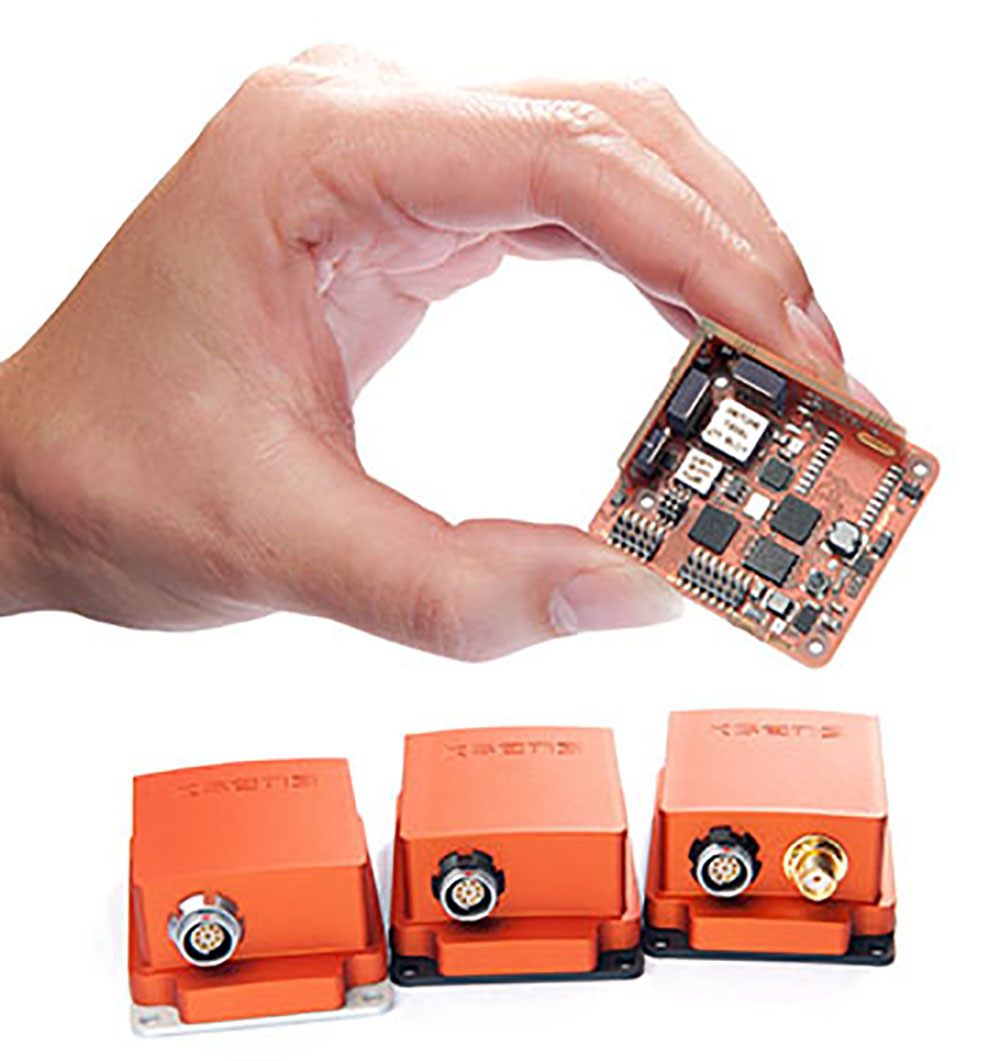
\includegraphics[height=0.45\textheight]{05.instrumentos.giroscopicos.imagenes/05.06.central.giroscopica/05-06-ahrs_.jpg}

    {\tiny Fuente: \url{https://www.xsens.com/products/mti-100-series/}}

\end{column}
\begin{column}{0.4\textwidth}
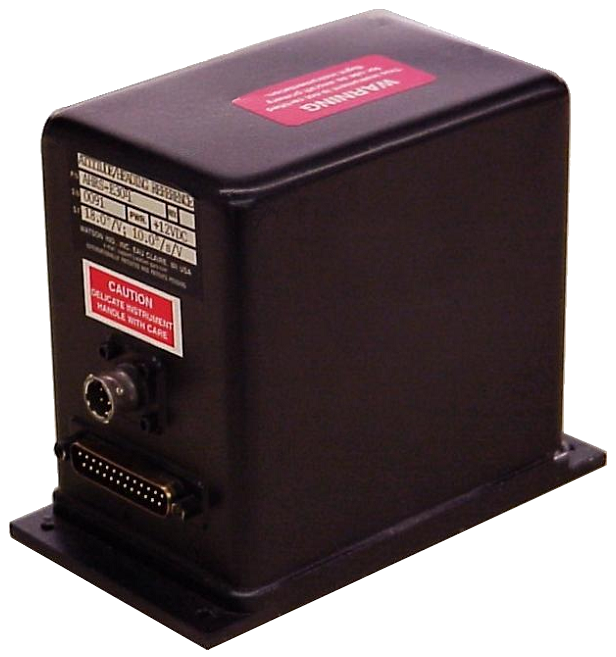
\includegraphics[height=0.45\textheight]{05.instrumentos.giroscopicos.imagenes/05.06.central.giroscopica/05-06-AHRS-E304_product.png}

      {\tiny Fuente: \url{https://watson-gyro.com/?s=ahrs} }

\end{column}
\end{columns}

\end{frame}

% \begin{frame}{AFCS}
  
%   \begin{block}{Automatic Flight Control System}
%     Es el sistema base de control de las futuras aeronaves no tripuladas, se basa en los siguientes conceptos:
%     \begin{itemize}
%     \item Equipar un piloto automático que controle la navegación
%     \item Enviar y recibir información de telemetría y comandos a/de la estación terrestre
%     \item Controlar los sistemas eléctrico, propulsivo y de presurización de la aeronave.
%     \end{itemize}
% Debe cumplir las siguientes funciones:
% \begin{itemize}
% \item Aceptar órdenes de la estación terrestre y realizar los comandos en la aeronave.
% \item  Monitorizar los subsistemas y detectar fallos.
% \item  Determinar altitud y posición y proveer de estos datos al piloto automático.
% \item  Seguir el algoritmo guía.
% \item  Poder retornar a casa en caso de emergencia. 
% \end{itemize}
%   \end{block}

% \end{frame}

% \begin{frame}

% 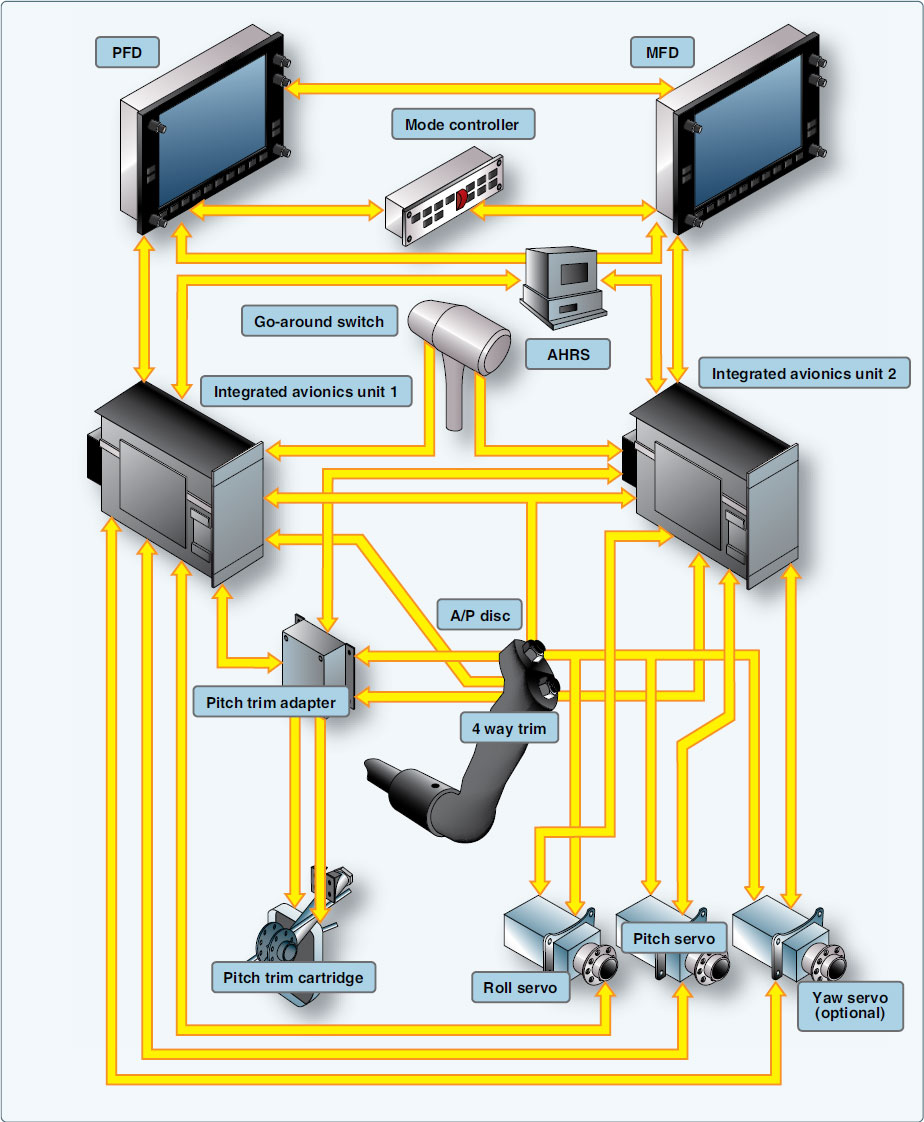
\includegraphics[height=0.85\textheight]{05.instrumentos.giroscopicos.imagenes/05.06.central.giroscopica/05-06-AFCS_0001.jpg}

% {\tiny Fuente: \url{https://www.flight-mechanic.com/automatic-flight-control-system-afcs-and-flight-director-systems/}}
% \end{frame}